% fapolicyd Power Users
% Goal: after this talk you can install, configure, debug, triage.
% Sparse slides. Practice drills: EXERCISES.md
\documentclass[aspectratio=169,11pt]{beamer}

\IfFileExists{beamerthememetropolis.sty}{%
  \usetheme{metropolis}%
}{%
  \usetheme{default}%
  \setbeamertemplate{navigation symbols}{}%
}

\usepackage[T1]{fontenc}
\usepackage{booktabs}
\usepackage{hyperref}
\usepackage{tikz}
\usetikzlibrary{arrows.meta,positioning}

\title{fapolicyd for Power Users}
\subtitle{Leave able to configure and debug it}
\author{SELinux Development Team Workshop}
\date{\today}

\begin{document}

\begin{frame}
  \titlepage
\end{frame}

%---------------------------------------------------------------------
\begin{frame}{Goal of this talk}
  After these slides (+ live demo) you can:
  \begin{itemize}
    \item Install and verify fapolicyd
    \item Trust unpackaged software
    \item Add a \texttt{rules.d} drop-in safely
    \item Debug a denial and triage AVC vs FANOTIFY
  \end{itemize}
\end{frame}

\begin{frame}{How we get there}
  \begin{itemize}
    \item \textbf{Why} --- trust layer beside MAC (short)
    \item \textbf{What} --- trust DB, rules, integrity
    \item \textbf{Configure} --- exact workflows
    \item \textbf{Live} --- one end-to-end example
  \end{itemize}
\end{frame}

\begin{frame}{At home = practice, not first contact}
  \begin{itemize}
    \item Config knowledge is \emph{in this deck}
    \item \texttt{EXERCISES.md} drills muscle memory
    \item Showcases = present later, not learn first
  \end{itemize}
\end{frame}

\begin{frame}{Agenda}
  \tableofcontents
\end{frame}

%=====================================================================
\section{Why}

\begin{frame}{Beside SELinux, not instead}
  \begin{itemize}
    \item SELinux: \emph{behavior} (labels / domains)
    \item fapolicyd: \emph{known artifact?} (trust / provenance)
    \item Same action can hit AVC, FANOTIFY, or both
  \end{itemize}
\end{frame}

\begin{frame}{What you gain / limits}
  \begin{itemize}
    \item Block unpackaged home / tmp / \texttt{/opt} code
    \item Stop \texttt{ld.so} smuggling (\texttt{pattern=ld\_so})
    \item Whitelist by trust --- not ``it has \texttt{bin\_t}''
    \item Limits: root can disable it; not a MAC substitute
  \end{itemize}
\end{frame}

%=====================================================================
\section{What you configure}

\begin{frame}{Three places that matter}
  \begin{enumerate}
    \item Trust DB --- known files
    \item \texttt{rules.d/} --- policy
    \item \texttt{fapolicyd.conf} --- mode / integrity / tuning
  \end{enumerate}
\end{frame}

\begin{frame}{Architecture (for intuition)}
  \centering
  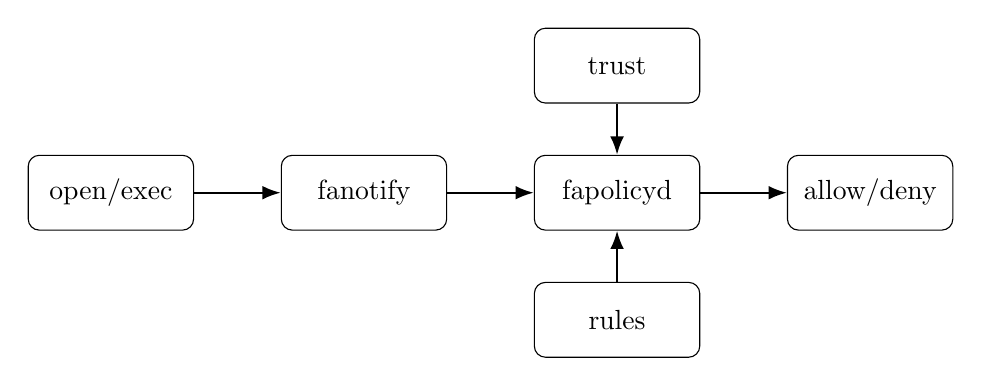
\begin{tikzpicture}[
    box/.style={draw,rounded corners,align=center,minimum height=0.95cm,minimum width=2.1cm},
    arr/.style={-{Latex},thick}
  ]
    \node[box] (app) {open/exec};
    \node[box,right=1.1cm of app] (fan) {fanotify};
    \node[box,right=1.1cm of fan] (dap) {fapolicyd};
    \node[box,above=0.65cm of dap] (trust) {trust};
    \node[box,below=0.65cm of dap] (rules) {rules};
    \node[box,right=1.1cm of dap] (dec) {allow/deny};
    \draw[arr] (app) -- (fan);
    \draw[arr] (fan) -- (dap);
    \draw[arr] (trust) -- (dap);
    \draw[arr] (rules) -- (dap);
    \draw[arr] (dap) -- (dec);
  \end{tikzpicture}
\end{frame}

\begin{frame}{Hard rule}
  \centering
  \vspace{1.2em}
  {\Large Never strace / gdb the daemon}
  \vspace{0.8em}

  SIGSTOP $\Rightarrow$ system-wide deadlock
\end{frame}

\begin{frame}{Trust --- two backends}
  \begin{itemize}
    \item \texttt{rpmdb} --- from RPM (auto via plugin)
    \item \texttt{filedb} --- you add in \texttt{trust.d/}
  \end{itemize}
\end{frame}

\begin{frame}[fragile]{Trust --- entry}
  \begin{semiverbatim}
filedb /opt/app/bin/x  SIZE  SHA256
  \end{semiverbatim}
  \vspace{0.6em}
  Rules see \texttt{trust=1} or \texttt{trust=0}
\end{frame}

\begin{frame}{Rules --- recipe}
  \centering
  \vspace{1em}
  {\large\texttt{decision permission subject : object}}
  \vspace{1em}

  First match wins
\end{frame}

\begin{frame}[fragile]{Shipped: \texttt{pattern=ld\_so}}
  \begin{semiverbatim}
deny_audit perm=any pattern=ld_so : all
  \end{semiverbatim}
  \vspace{0.6em}
  Trusted loader does \emph{not} bless an untrusted ELF.\\
  (\texttt{ld.so ./evil} still denied)
\end{frame}

\begin{frame}{Rules --- where they live}
  \begin{itemize}
    \item Edit \texttt{/etc/fapolicyd/rules.d/NN-name.rules}
    \item \texttt{fagenrules} builds \texttt{compiled.rules}
    \item Never hand-edit compiled output
  \end{itemize}
\end{frame}

\begin{frame}{Default policy}
  \begin{itemize}
    \item Shipped set: \texttt{known-libs}
    \item Trusted stuff mostly works
    \item Unpackaged execute/open of code $\rightarrow$ deny
  \end{itemize}
\end{frame}

\begin{frame}{Integrity in conf}
  \begin{itemize}
    \item \texttt{none} --- default
    \item \texttt{size} --- good first step
    \item \texttt{sha256} --- costly; plan capacity
  \end{itemize}
\end{frame}

%=====================================================================
\section{Configure}

\begin{frame}{Workflow A --- install}
  \begin{enumerate}
    \item \texttt{dnf install fapolicyd fapolicyd-selinux}\\
          \texttt{rpm-plugin-fapolicyd}
    \item Ensure $\ge$ 1 audit rule exists
    \item \texttt{systemctl enable --now fapolicyd}
  \end{enumerate}
\end{frame}

\begin{frame}{Workflow A --- verify}
  \begin{itemize}
    \item \texttt{fapolicyd-cli --check-status}
    \item \texttt{fapolicyd-cli --list | head}
    \item Expect: Permissive false, trust entries $>$ 0
  \end{itemize}
\end{frame}

\begin{frame}{Audit rule (why)}
  \begin{itemize}
    \item Without any audit rule, \texttt{deny\_audit} is quiet
    \item Dummy: \texttt{auditctl -w /etc/shadow -p w}
    \item Watch $\neq$ chmod --- permissions unchanged
  \end{itemize}
\end{frame}

\begin{frame}{Workflow B --- trust an /opt app}
  This is the default remediation.
\end{frame}

\begin{frame}[fragile]{Trust /opt --- commands}
  \begin{semiverbatim}
fapolicyd-cli --file add /opt/myapp \\
  --trust-file myapp
fapolicyd-cli --update
  \end{semiverbatim}
\end{frame}

\begin{frame}{Trust /opt --- remember}
  \begin{itemize}
    \item \texttt{--file add} writes \texttt{trust.d/}
    \item \texttt{--update} reloads the daemon DB
    \item Prefer this over allow rules
  \end{itemize}
\end{frame}

\begin{frame}[fragile]{Inspect trust}
  \begin{semiverbatim}
fapolicyd-cli --dump-db | grep myapp
ls /etc/fapolicyd/trust.d/
  \end{semiverbatim}
\end{frame}

\begin{frame}{Workflow C --- custom rule}
  Use only when you need \emph{who} / \emph{how},\\
  not just ``is it known?''
\end{frame}

\begin{frame}[fragile]{Custom rule --- drop-in}
  \begin{semiverbatim}
# /etc/fapolicyd/rules.d/55-ping.rules
allow perm=any gid=wheel :
  trust=1 path=/usr/bin/ping
deny_audit perm=execute all :
  trust=1 path=/usr/bin/ping
  \end{semiverbatim}
\end{frame}

\begin{frame}[fragile]{Custom rule --- apply}
  \begin{semiverbatim}
fagenrules
fapolicyd-cli --check-rules --lint
systemctl reload fapolicyd
fapolicyd-cli --list | grep ping
  \end{semiverbatim}
\end{frame}

\begin{frame}{Custom rule --- safety}
  \begin{itemize}
    \item Number file so it sits \emph{above} deny-all
    \item Bad reload keeps previous ruleset
    \item Keep drop-ins sparse
  \end{itemize}
\end{frame}

\begin{frame}{Workflow D --- conf knobs}
  File: \texttt{/etc/fapolicyd/fapolicyd.conf}
\end{frame}

\begin{frame}{Conf --- soak then enforce}
  \begin{itemize}
    \item \texttt{permissive = 1} while learning / soaking
    \item Watch denials, fix trust/rules
    \item Then \texttt{permissive = 0} + restart
  \end{itemize}
\end{frame}

\begin{frame}{Conf --- integrity}
  \begin{itemize}
    \item Start with \texttt{integrity = size} if you want more
    \item Avoid jumping straight to sha256
  \end{itemize}
\end{frame}

\begin{frame}{Decision tree --- denied?}
  \begin{enumerate}
    \item \texttt{ausearch -m AVC} $\rightarrow$ SELinux
    \item \texttt{ausearch -m FANOTIFY -i} $\rightarrow$ fapolicyd\\
          {\small (compact events often lack path --- use \texttt{--debug-deny})}
    \item Neither / unclear $\rightarrow$ debug-deny
  \end{enumerate}
\end{frame}

\begin{frame}{Dual stack}
  \begin{itemize}
    \item One binary can hit \textbf{both} AVC and FANOTIFY
    \item Wrong label $\rightarrow$ AVC; untrusted $\rightarrow$ FANOTIFY
    \item Fix each layer separately (label/policy vs trust/rules)
  \end{itemize}
\end{frame}

\begin{frame}{If FANOTIFY deny}
  \begin{itemize}
    \item Should be known software? $\rightarrow$ trust + \texttt{--update}
    \item Who/how exception? $\rightarrow$ \texttt{rules.d} drop-in
  \end{itemize}
\end{frame}

\begin{frame}{Debug loop (1/2)}
  \begin{enumerate}
    \item \texttt{systemctl stop fapolicyd}
    \item \texttt{fapolicyd --permissive --debug-deny}
    \item Reproduce $\rightarrow$ \texttt{rule:N} \ldots \texttt{file=}
  \end{enumerate}
\end{frame}

\begin{frame}{Debug loop (2/2)}
  \begin{enumerate}
    \setcounter{enumi}{3}
    \item \texttt{fapolicyd-cli --list} $\rightarrow$ map N
    \item Fix trust or move allow above deny
    \item Restart service when done
  \end{enumerate}
\end{frame}

\begin{frame}{CLI cheat}
  \begin{itemize}
    \item Inspect: \texttt{--check-status}, \texttt{--list}, \texttt{--dump-db}
    \item Change: \texttt{--file add/delete}, \texttt{--update}
    \item Check: \texttt{--check-rules --lint}
  \end{itemize}
\end{frame}

\begin{frame}{Anti-patterns}
  \begin{itemize}
    \item Allow-list sprawl instead of trust
    \item Edit \texttt{compiled.rules}
    \item Assume SELinux allow $\Rightarrow$ fapolicyd allow
  \end{itemize}
\end{frame}

%=====================================================================
\section{Live}

\begin{frame}{We configure together}
  Install $\rightarrow$ deny clone of \texttt{ls} $\rightarrow$ trust it $\rightarrow$ allow\\[0.6em]
  {\large Run the binary as \texttt{fapo}, not root}
\end{frame}

\begin{frame}{Setup}
  \begin{itemize}
    \item \texttt{sudo demos/00-lab-prep.sh} $\rightarrow$ lands as \texttt{fapo}
    \item Or install + enable by hand, then \texttt{su - fapo}
  \end{itemize}
\end{frame}

\begin{frame}{Why not root?}
  \begin{itemize}
    \item Shipped: \texttt{allow perm=any uid=0 trust=1 : all}
    \item Root + trusted shell $\Rightarrow$ untrusted \texttt{/opt} often \textbf{allowed}
    \item Deny labs need workshop user \texttt{fapo}
  \end{itemize}
\end{frame}

\begin{frame}[fragile]{Deny (as fapo)}
  \begin{semiverbatim}
id -u    # must NOT be 0
sudo cp -a /usr/bin/ls /opt/fapo-workshop/my-ls
sudo chmod 755 /opt/fapo-workshop/my-ls
/opt/fapo-workshop/my-ls          # DENY
  \end{semiverbatim}
\end{frame}

\begin{frame}[fragile]{Configure fix (as fapo)}
  \begin{semiverbatim}
sudo fapolicyd-cli --file add \\
  /opt/fapo-workshop/my-ls --trust-file workshop
sudo fapolicyd-cli --update
/opt/fapo-workshop/my-ls          # ALLOW
  \end{semiverbatim}
\end{frame}

\begin{frame}{You just configured trust}
  \begin{itemize}
    \item Diagnosed untrusted execute
    \item Applied the standard fix
    \item Verified allow
  \end{itemize}
\end{frame}

%=====================================================================
\section{You leave able to}

\begin{frame}{Checklist}
  \begin{itemize}
    \item[$\square$] Install + verify status
    \item[$\square$] Trust an \texttt{/opt} tree
    \item[$\square$] Add / reload a rules drop-in
    \item[$\square$] Debug with \texttt{rule:N}
    \item[$\square$] Triage AVC vs FANOTIFY
  \end{itemize}
\end{frame}

\begin{frame}{Practice next}
  \begin{itemize}
    \item \texttt{EXERCISES.md} --- predict / do / answer
    \item \texttt{TAKE-HOME.md} --- cookbook reference
    \item \texttt{demos/showcases/} --- demo to others later
  \end{itemize}
\end{frame}

\begin{frame}{Discussion}
  \begin{itemize}
    \item Where on staff machines?
    \item How do we teach AVC vs FANOTIFY?
  \end{itemize}
\end{frame}

\begin{frame}{References}
  \begin{itemize}
    \item linux-application-whitelisting/fapolicyd
    \item RHEL Security hardening --- fapolicyd
    \item man: fapolicyd(8), rules(5), cli(8)
  \end{itemize}
\end{frame}

\begin{frame}
  \centering
  {\LARGE Questions}\\[1.2em]
  You should be able to configure it now.\\[0.6em]
  Drill with \texttt{EXERCISES.md}
\end{frame}

\end{document}
